\documentclass[tikz,border=12pt]{standalone}
\usepackage[T1]{fontenc}
\usepackage{mathpazo}
\usepackage{amsmath,amssymb}
\usetikzlibrary{arrows.meta, positioning, calc}

\definecolor{stblue}{HTML}{7B97AD}
\definecolor{rwgold}{HTML}{B8995E}
\definecolor{sage}{HTML}{7A9A7E}
\definecolor{dkbrown}{HTML}{3D3530}
\definecolor{wmgray}{HTML}{7B7067}
\definecolor{cream}{HTML}{F9F6F0}
\definecolor{border}{HTML}{D4C9B8}
\definecolor{terracotta}{HTML}{C47A6A}

\begin{document}
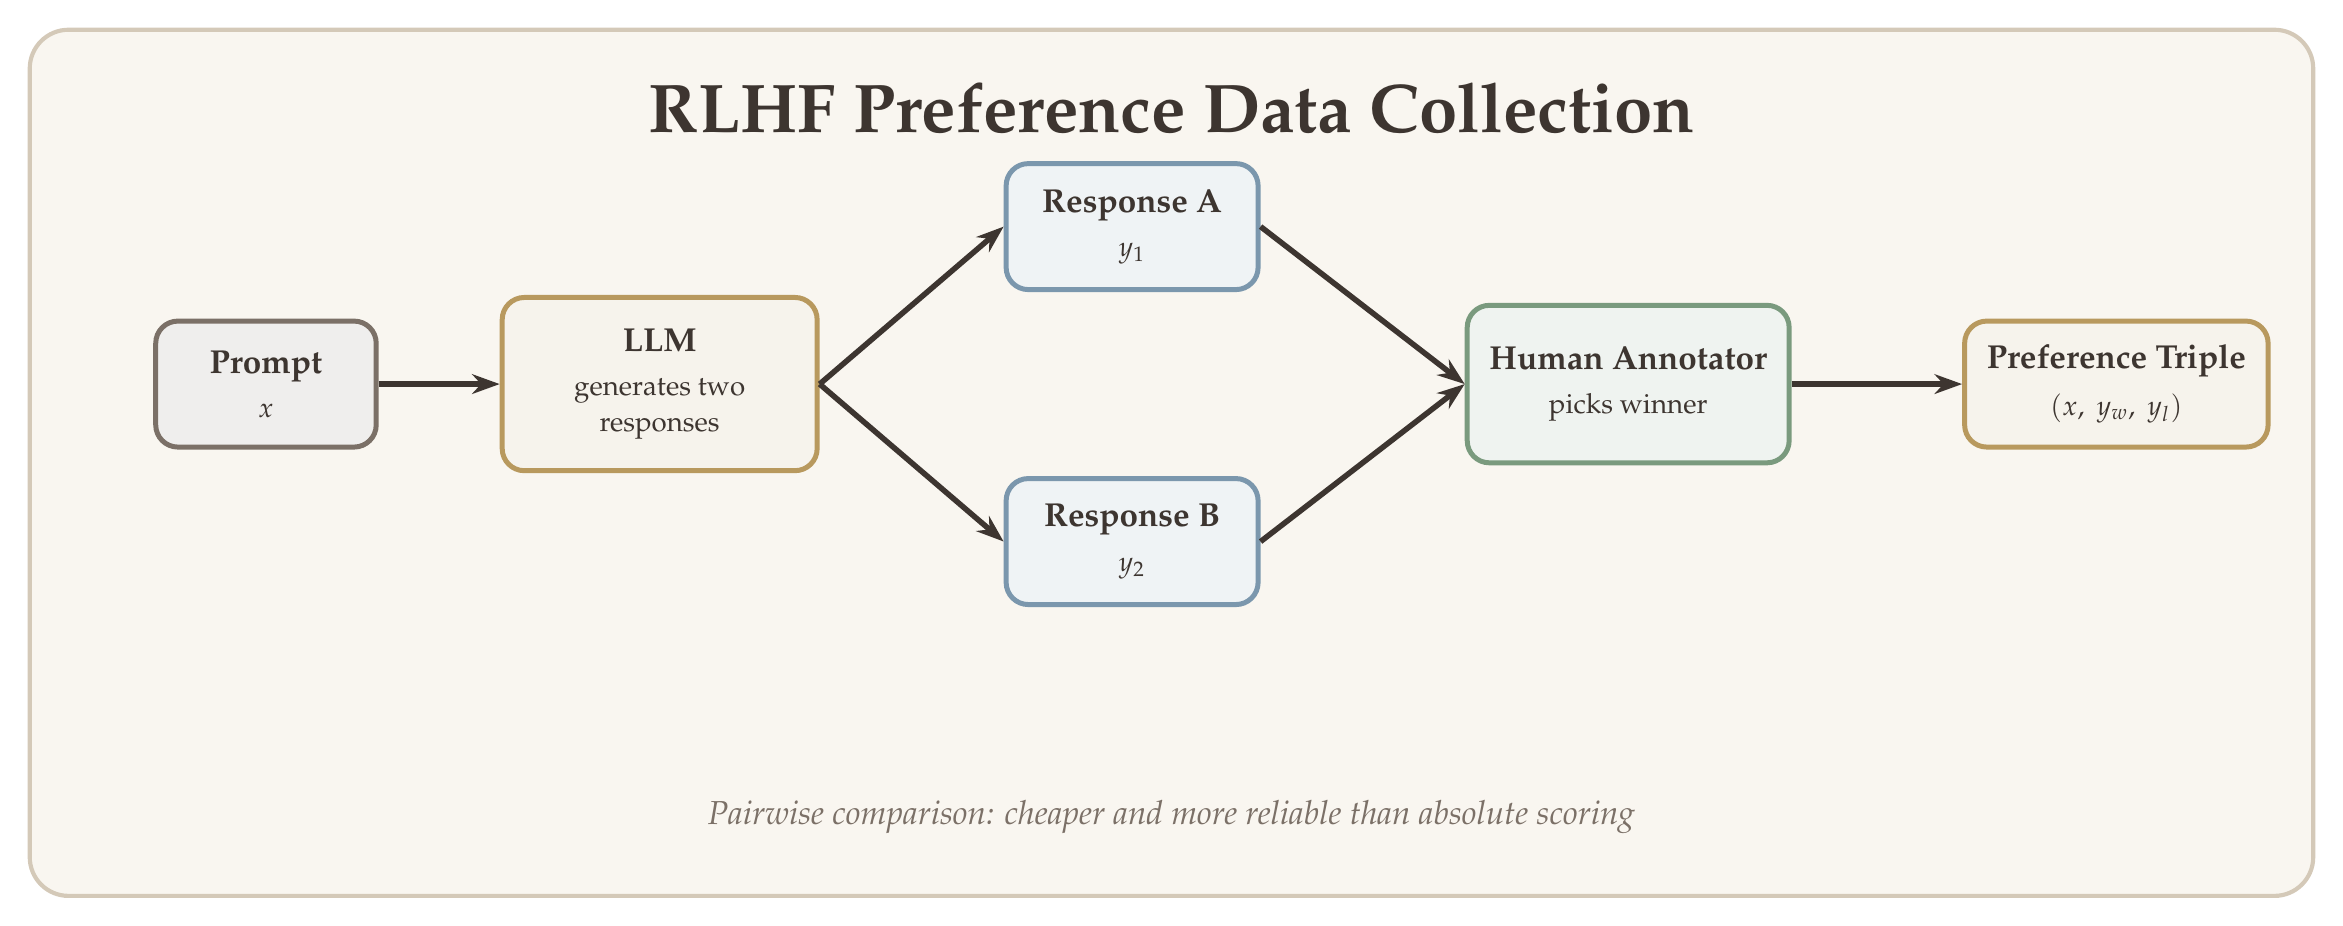
\begin{tikzpicture}[
  >={Stealth[length=3.5mm, width=2.5mm]},
  box/.style={draw=#1, line width=1.8pt, fill=#1!12, rounded corners=8pt,
    minimum height=16mm, font=\large, text=dkbrown, align=center, inner sep=8pt},
  arr/.style={->, line width=2pt, dkbrown},
]

% Background
\fill[cream, rounded corners=14pt] (-1.5,-3.5) rectangle (27.5,7.5);
\draw[border, rounded corners=14pt, line width=1.5pt] (-1.5,-3.5) rectangle (27.5,7.5);

% Title
\node[font=\Huge\bfseries, text=dkbrown] at (13,6.5)
  {RLHF Preference Data Collection};

% === Stage 1: Prompt ===
\node[box=wmgray, minimum width=28mm] (prompt) at (1.5,3)
  {\textbf{Prompt}\\[2pt] \normalsize $x$};

% === Stage 2: Model generates ===
\node[box=rwgold, minimum width=40mm, minimum height=22mm] (model) at (6.5,3)
  {\textbf{LLM}\\[2pt] \normalsize generates two\\[-1pt] \normalsize responses};

% Arrow: Prompt -> Model
\draw[arr] (prompt.east) -- (model.west);

% === Stage 3: Two responses branch out ===
\node[box=stblue, minimum width=32mm] (respA) at (12.5,5)
  {\textbf{Response A}\\[2pt] \normalsize $y_1$};
\node[box=stblue, minimum width=32mm] (respB) at (12.5,1)
  {\textbf{Response B}\\[2pt] \normalsize $y_2$};

% Diagonal arrows: Model -> responses
\draw[arr] (model.east) -- (respA.west);
\draw[arr] (model.east) -- (respB.west);

% === Stage 4: Human annotator ===
\node[box=sage, minimum width=38mm, minimum height=20mm] (human) at (18.8,3)
  {\textbf{Human Annotator}\\[2pt] \normalsize picks winner};

% Diagonal arrows: responses -> annotator
\draw[arr] (respA.east) -- (human.west);
\draw[arr] (respB.east) -- (human.west);

% === Stage 5: Preference triple ===
\node[box=rwgold, minimum width=38mm] (pref) at (25,3)
  {\textbf{Preference Triple}\\[3pt] \normalsize $(x,\; y_w,\; y_l)$};

% Arrow: annotator -> triple
\draw[arr] (human.east) -- (pref.west);

% === Bottom annotation ===
\node[font=\large\itshape, text=wmgray] at (13,-2.5)
  {Pairwise comparison: cheaper and more reliable than absolute scoring};

\end{tikzpicture}
\end{document}
